% !tex root = ../Thesis.tex

\section{Problem Statement}

Musicians are faced with the challenge of creating good music. This comes down to
controlling many different qualities of the sound they produce. The tempo, rhythm,
pitch and volume are some examples of these qualities. They often make mistakes
under the pressure of live performances or even when making studio recordings.
Pitch is specifically hard to control for vocalists or musicians who play
instruments in the horn or fretless string families. Errors in pitch accuracy are
known as intonation errors and effect both the harmonic and melodic structure of
the music, degrading it's aesthetic appeal. Since all the efforts of the musician
culminates in a sound wave, it is subject to analysis and manipulation by the
tools, algorithms and effects developed in the field of signal processing.

Pitch correction is an effect applied to audio that attempts to fix errors in
intonation. This involves minimally changing the waveform to have the desired
pitch while retaining all the other qualities of the waveform. This effect is
mostly discussed in the context of music, where pitch is considered an important
quality, but some considerations in other fields such as speech comprehension can
be conceived.

\begin{figure}[b!]
	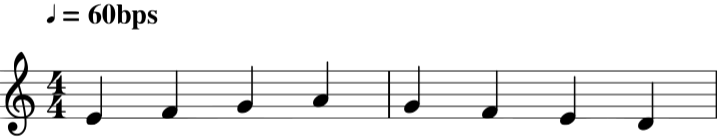
\includegraphics[width=\textwidth]{MusicNotation}
	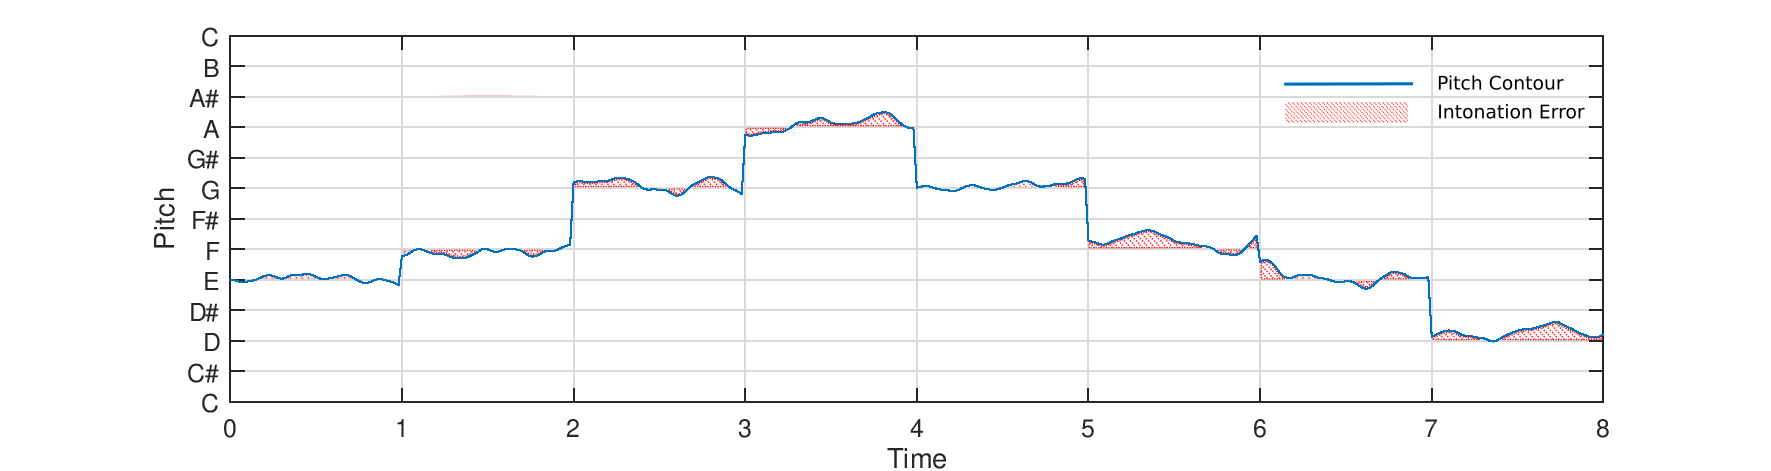
\includegraphics[width=\textwidth,trim={3.5cm 0cm 2.8cm 0cm}]
	{IntonationError}
	\caption{Illustration of Intonation Errors in a Pitch Contour Diagram}
	\label{fig:IntonationError}
\end{figure}

Figure \ref{fig:IntonationError} shows an example of what is meant by errors in
intonation. The graph is a pitch contour diagram, plotting the quality of pitch
over time. One of the goals of the musician is to make the pitch contour follow
the pitch indicated by music notation as closely as possible during the duration
of the note. The red regions indicate errors in intonation, i.e.  the times which
the pitch contour does not follow the pitch indicated by the note. The goal of
pitch correction is to alter the waveform to minimize these regions of intonation
error while minimally affecting other properties of the waveform.

Pitch correction is difficult because it fundamentally require two non-trivial
operations. These operations are pitch detection and pitch shifting. What's more
is that these operations need to be efficiently implemented in order to allow for
real time, minimal latency throughput for when pitch correction is needed for a
live performance.

There are many different algorithms for pitch detection, each optimized for
different situations. In the context of monophonic audio, the pitch detector needs
to have robust performance in the presence of noise and prominent harmonics. The
pitch shifter is fundamentally a harder problem to solve. This is explained by
giving a naive example of how one could consider approaching pitch shifting.  One
could consider just playing the audio faster or slower, depending on the type of
shift required. While this does successfully shift the pitch it alters some other
qualities of the audio as well. The most important of which is duration, which
also affects the tempo and rhythm. Another quality that this approach would alter
is the formant structure of the sound. This is related to the harmonics of the
sound and is explained later in the report. Altering this quality essentially
comes down to the sound having an unnatural feeling to it.

\vspace{4mm}\noindent
The desire to have a pitch correction system can be summarised in a few use cases:
\begin{itemize}
\item
A vocalist records some tracks at a recording studio. The whole song is perfect
except for one out of tune note. This is only realised a few days later in the
mixing phase of producing the song. Going back to the recording studio would be
inconvenient and expensive. Having a tool to simply fix the intonation of this
note without the need to involve the vocalist or recording studio would be
strongly desired.
\item
A poor mumble rapper, call him Lil Pump, needs to deliver an important message, in
the form of his latest song, to his followers in a live performance. Unfortunately
he's not very talented and cannot sing in tune. A live pitch correction system,
that would make his voice sound tolerable, would help him deliver this important
message.
\item
A computer gaming company wants to create a game with an evil artificial
intelligence antagonist. This character needs to have an eerily ``perfect'' voice.
A system that can apply an effect on a human voice to sound perfectly in tune may
create the desired effect.
\end{itemize}

\section{History of Audio Pitch Correction}

One of the first occurrences of pitch manipulation in music, at least the first
occurrence that was found by the author, was of a song\footnote{The Chipmunk Song:
\url{https://www.youtube.com/watch?v=b3p7tZw6Mps}} called ``The Chipmunk Song''
from the animated music group ``Alvin and the Chipmunks''. The goal was to raise
the pitch of the voice of a singer to sound an octave higher than his actual
voice. This was accomplished by recording the song at half the wanted tempo and
playing back the recording at twice the speed when mixing. The technology used in
audio recordings was still analog tape recordings and the whole process was done
using these tapes. The effect of speeding up a recording to achieve a pitch shift
became known as the ``Chipmunk Effect''. The approach earned the group two Grammy
awards\footnote{\url{https://www.grammy.com/grammys/artists/ross-bagdasarian-sr}}
in 1958.

In 1977 Eventide introduced a new product, the Eventide H949
Harmonizer\footnote{\url{https://www.eventideaudio.com/products/clockworks-legacy/harmonizer/h949-harmonizer}},
capable of incremental pitch shifting. This was sold as a ``de-glitch pitch
shifter'' and was intended to be used to fix intonation errors and add
harmonization effects after recording. Other features commonly used was to stretch
the time of radio recordings of advertisements to be an exact duration without
affecting the pitch.  The pitch shifting was implemented using single side-band
modulation techniques and was done digitally.

\begin{figure}[h]
	\centering
	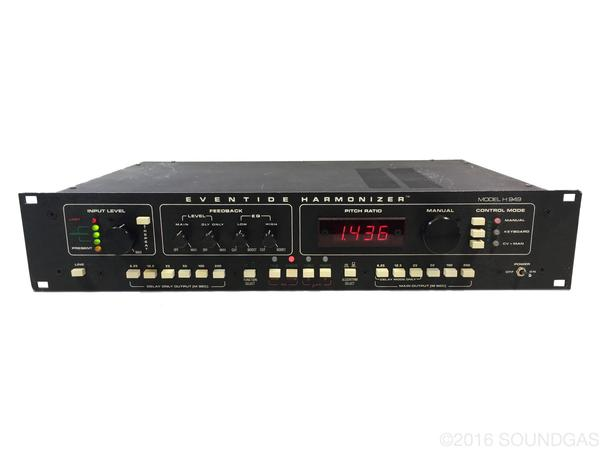
\includegraphics[width=0.9\textwidth,trim={0mm 55mm 0mm 55mm},clip]
	{EventideH949}
	\caption{Eventide H949 Harmonizer Rack Mounted Unit}
	\label{fig:EventideH949}
\end{figure}

In 1996 Andy Hildebrand, an electrical engineer, was investigating seismic data
when he realised that the same techniques he was using to investigate the data
could be used to alter the pitch of audio files. His techniques for detecting
pitch, using a simplification of the autocorrelation function, was considered
superior to the state of the art at that
time\footnote{\url{https://priceonomics.com/the-inventor-of-auto-tune}}. He
implemented the first version of his pitch correcting algorithm on his Macintosh
computer. His first demonstration was considered a success and the company
``Antares Audio'' was founded. A patent was filed in 1997 for a ``Pitch detection
and intonation correction apparatus and method''. They created a product called
``AutoTune'' which was popularised in 1998 by Cher in her song ``Believe'' which
made heavy use of the AutoTune pitch correction effect. AutoTune was the first
product capable of automatic real time pitch correction\cite{AutoTunePatent}.

\begin{figure}[h]
	\centering
	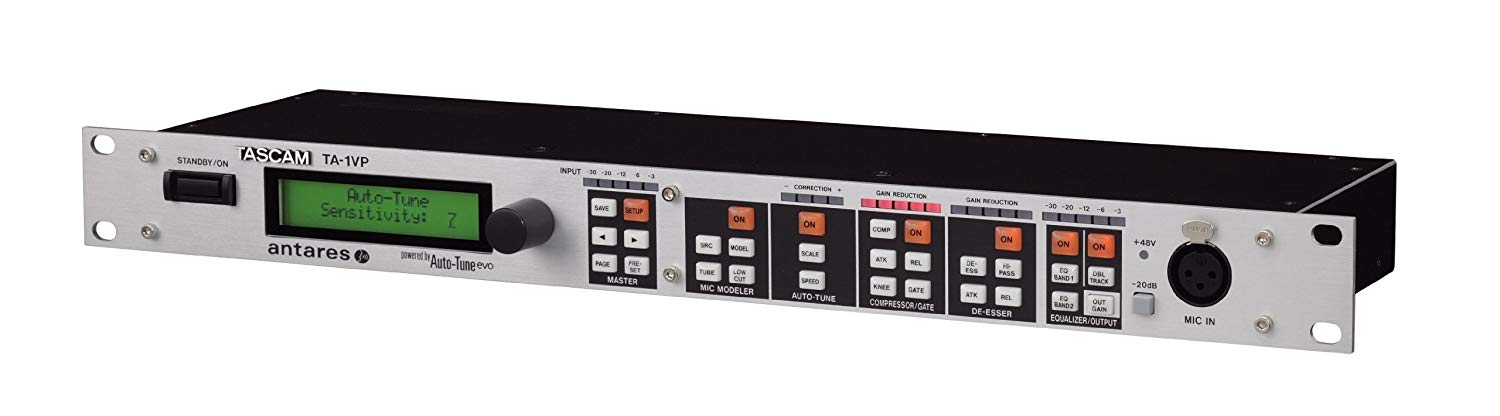
\includegraphics[width=0.9\textwidth,trim={30mm 20mm 30mm 30mm},clip]
	{AutoTuneRack}
	\caption{AutoTune Rack Mounted Unit}
	\label{fig:AutoTuneRack}
\end{figure}

AutoTune comes in a rack mounted unit for live performances shown in figure
\ref{fig:AutoTuneRack} or as a VST plugin. The software has evolved to allow for
many more features than the original pitch correction effect that the name
suggests. Modern AutoTune is still considered the state of the art product by
audio engineers.

In 2009 Tom Baran, an electrical engineer, wrote an open source pitch corrector.
This pitch corrector was written in the C programming language as a VST (Virtual
Studio Technology) plugin. At least two ports have been written and are up on
GitHub. The fact that this project is open source allows for inspection of the
code and provides insight in what design choices has been made. It uses an
autocorrelation approach to find the pitch, a PSOLA algorithm to shift the pitch
and a cubic spline interpolation algorithm for re-sampling\cite{AutoTalent}.

Finally Smule, a mobile phone application, was released in 2013. It's an
application for amateur singers to record themselves singing songs and sharing the
recordings on social media. The application features a pitch correction effect to
improve the quality of the recording before it is shared. This pitch correction is
done based on knowing what the harmony of the current note should be since it uses
a pre-recorded backing track. A patent was filled by Smule in 2011 for
``Pitch-correction of vocal performance in accord with score-coded
harmonies''\cite{SmulePatent}.

\section{Approach Taken}

The report follows the follow ng structure, starting with the literature review
chapter. The literature review starts with investigates music theory, defining the
concepts required for pitch correction and fundamentally answering the question of
what is considered correct. This is done by using the concept of a tuning system
to create a list of correct frequencies. Next, the pitch correction structure as a
whole is investigated and an idea of the required modules are formed. The
important modules are then investigate further, finalizing the literature review.


Thereafter, the implementation chapter discusses how the project was put together.
Assessment metrics are rigorously defined that can measure the success or failure
of a given pitch correcting system. These metrics aim to measure the pitch
accuracy improvement the system provides and the distortion caused by the system.
Thereafter a modular design is proposed for the pitch corrector, shown in figure
\ref{fig:PitchCorrectorFlowDiagramInto}.

\begin{figure}[h!]
\centering
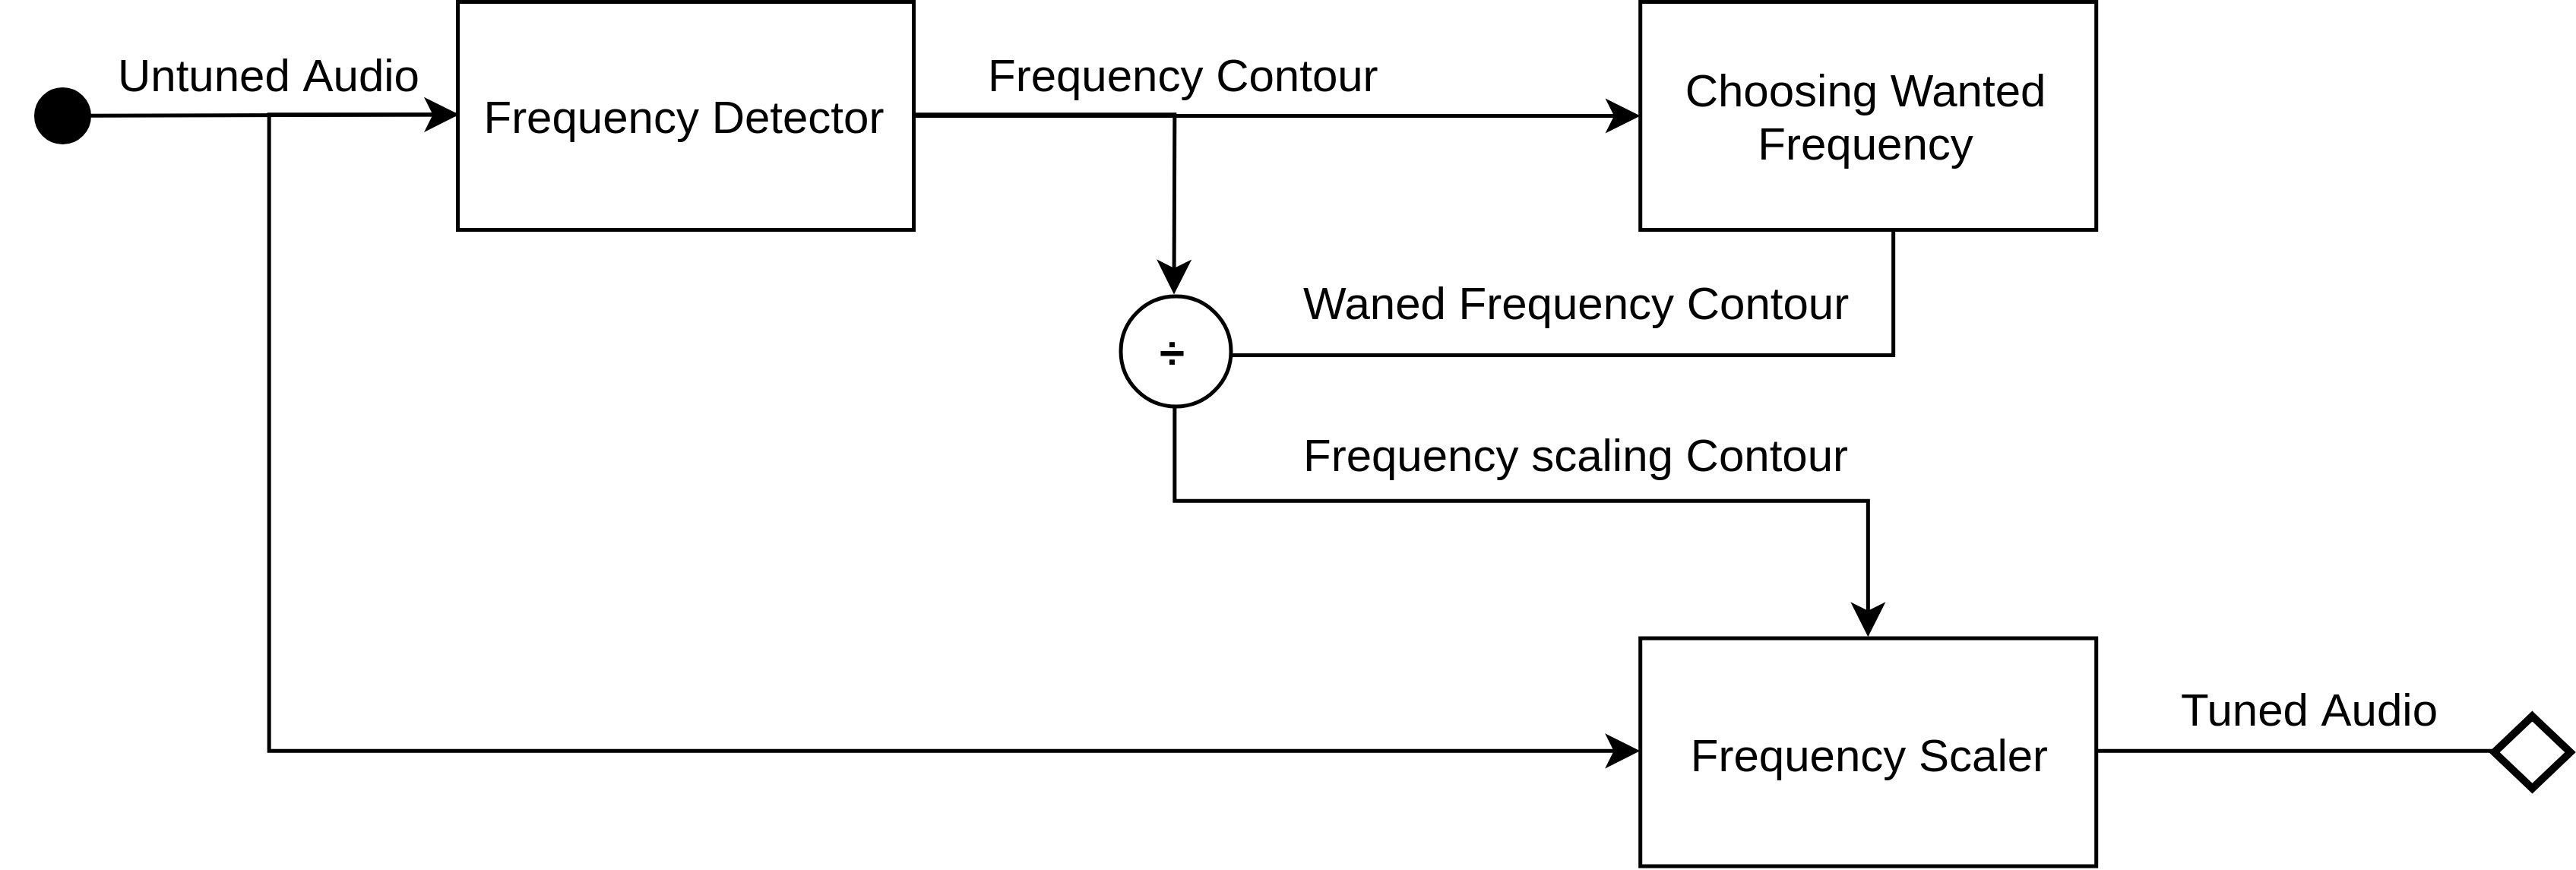
\includegraphics[width=\textwidth]{PitchCorrectorFlowDiagram}
\caption{Flow Diagram of Pitch Corrector}
\label{fig:PitchCorrectorFlowDiagramInto}
\end{figure}

Two implementations for the frequency detection modules are created and described.
One based on the zero-crossing method and the other based on the autocorrelation
approach. They were tested for noise robustness in the results chapter. The
zero-crossing method required a signal to noise ratio of 4.5db while the
autocorrelation method required a signal to noise ratio of 17.8db.

Two implementations for the frequency scaler were created and described. A simple
overlap and add method and a phase vocoder approach was implemented. Basic tests
were run to compare the two approaches and roughly determine their pitch
resolution. It was found that the phase vocoder approach had sufficient pitch
resolution, acceptable for pitch correction, while the simple overlap and add
approach did not.

The results chapter contains the results of the evaluation metrics defined in the
implantation chapter. These rigorous metrics were only run on one combination of
sub-modules, the zero-crossing method approach as the frequency detector and the
phase vocoder as the frequency scaler. The metrics found that this combination
produced a pitch accuracy improvement factor of 4.38 and a similarity of 44\% to
the original signal. A demo contour diagram is shown of how this system performs
with a real vocal recording. Figure \ref{fig:DemoIntro} shows the pitch contours
of the demo.

\begin{figure}[h]
	\center
	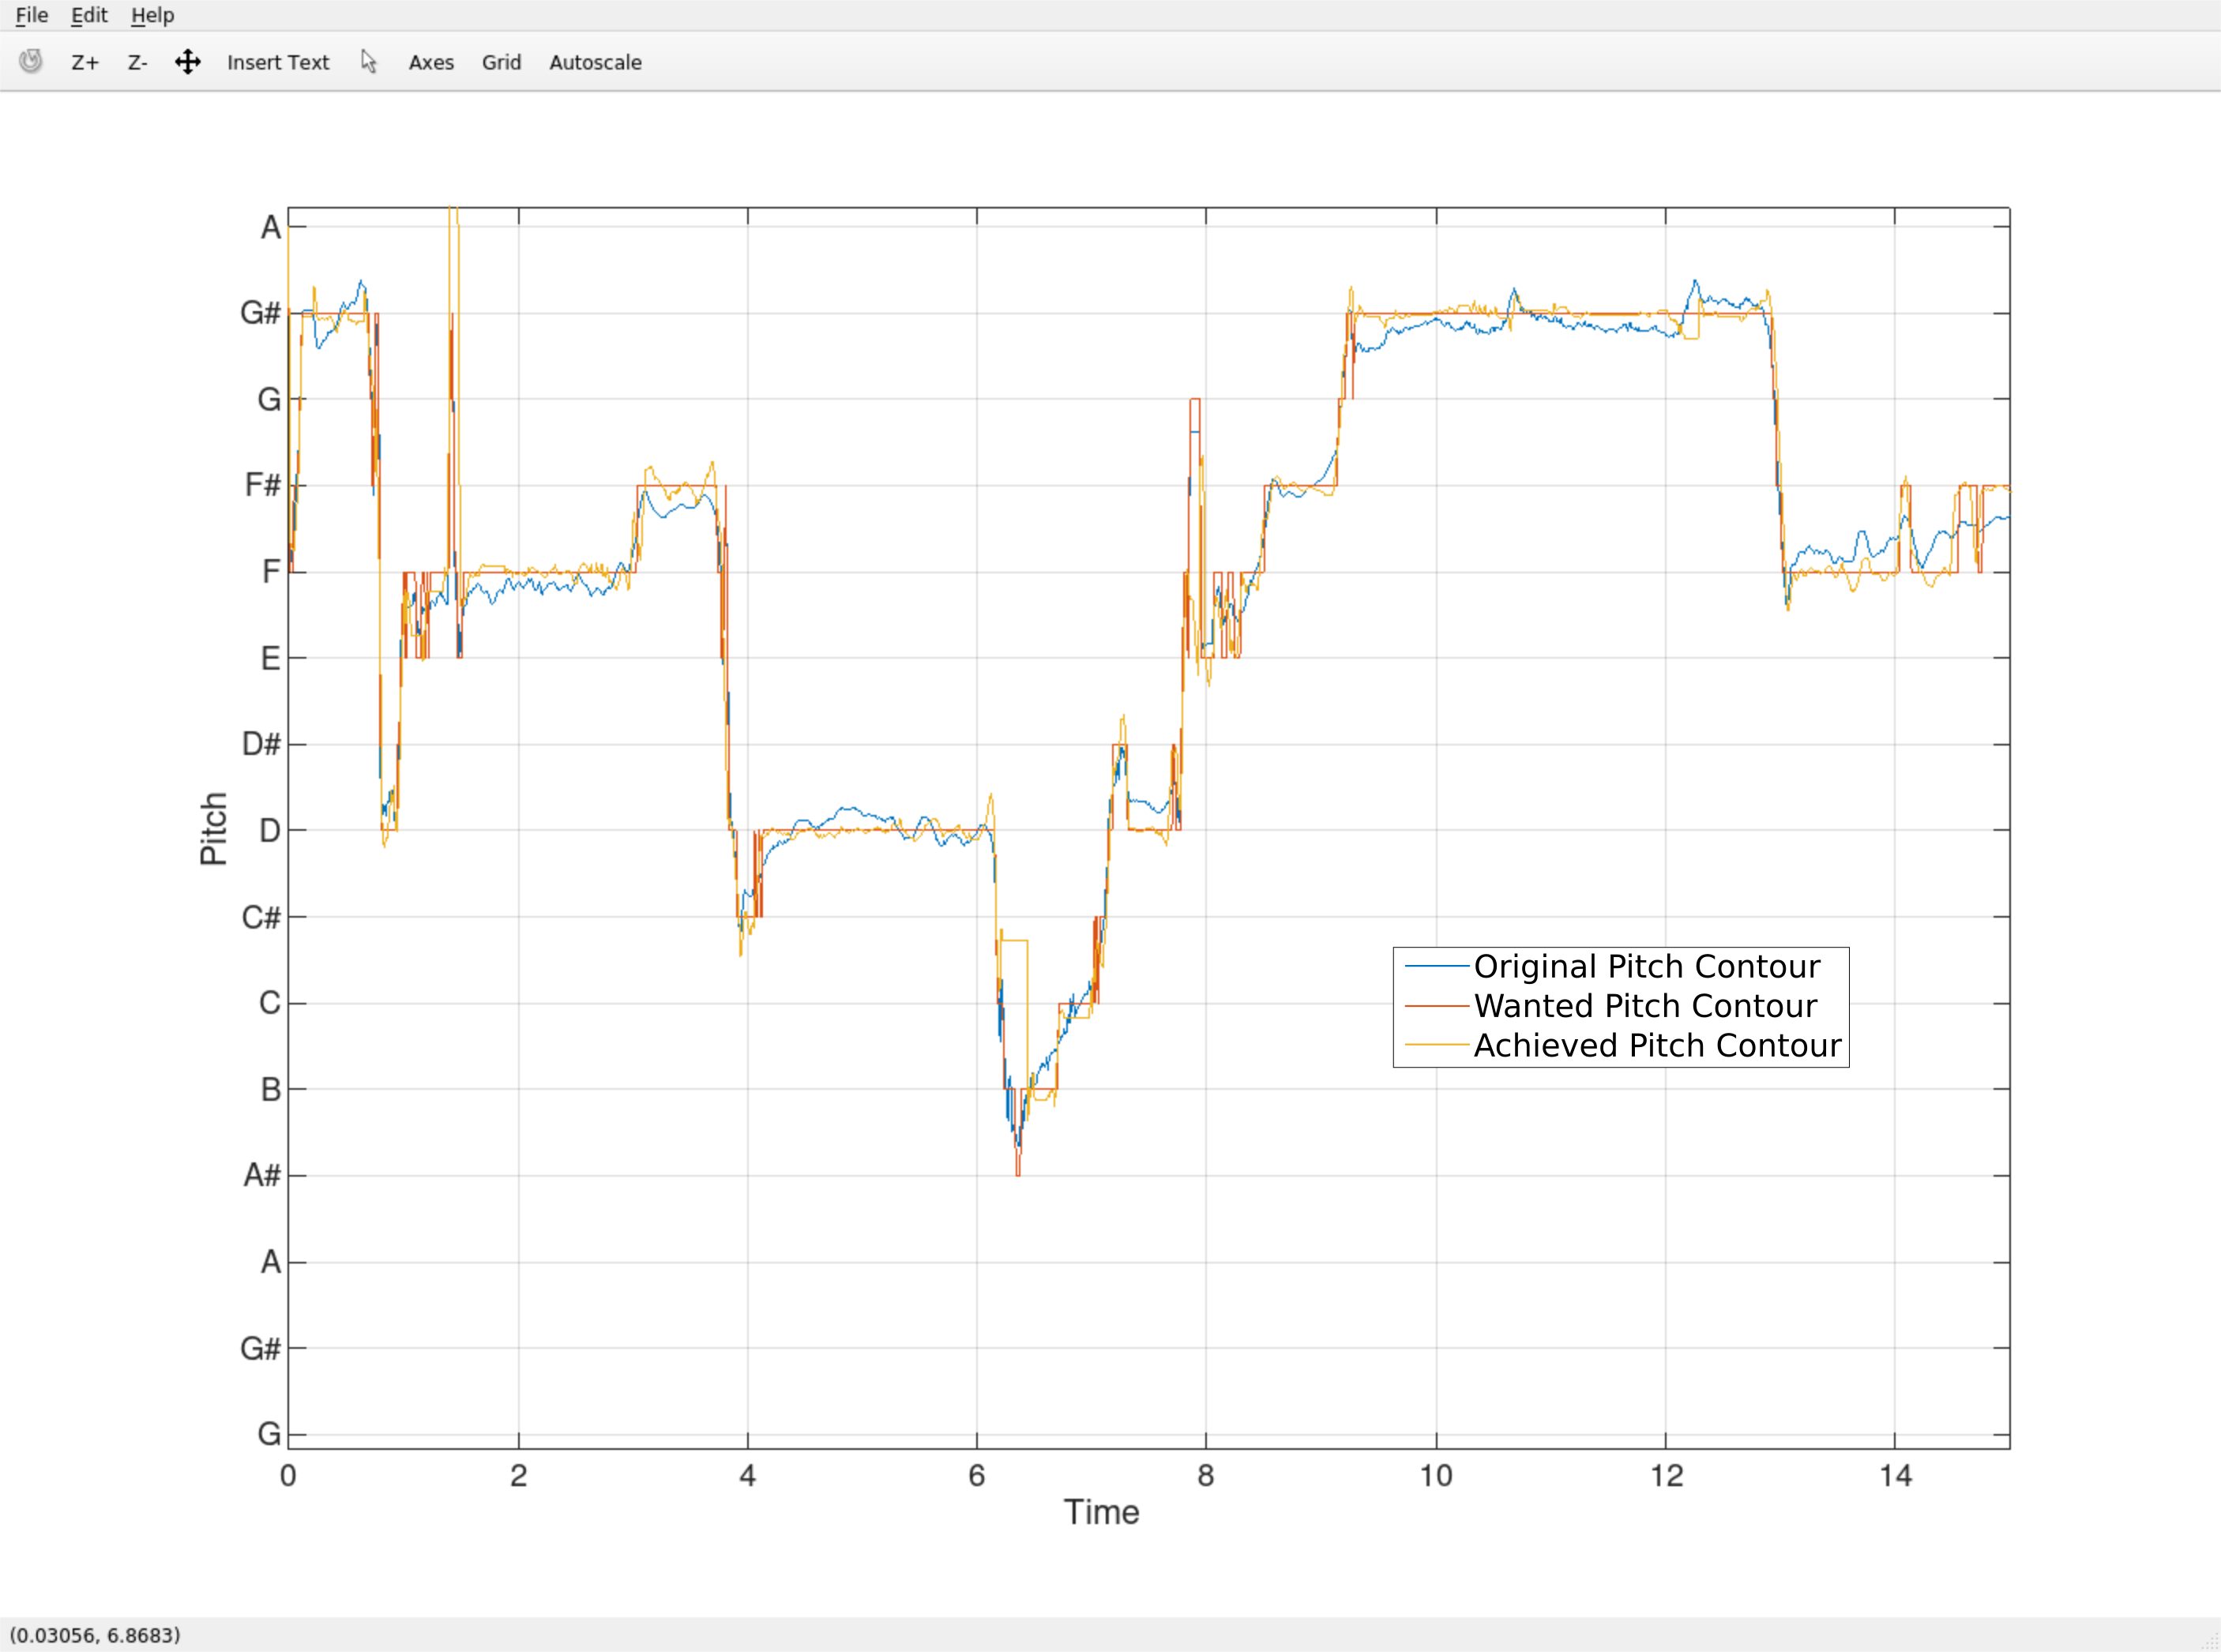
\includegraphics[width=\textwidth,trim={3.2cm 2cm 3cm 3cm},clip]
	{LiveDemo}
	\caption{Vocal recording demonstration of pitch correction}
	\label{fig:DemoIntro}
\end{figure}

The report concludes to say that the system, as it stand currently, is not capable
of non-cherry picked data and further investigation and development is required.
Recommendations are given on what such an investigation needs to consider and
investigate first.
